[216~v\textsuperscript{o}] 
\pend 
\vspace{2em}
\pstart
\centering
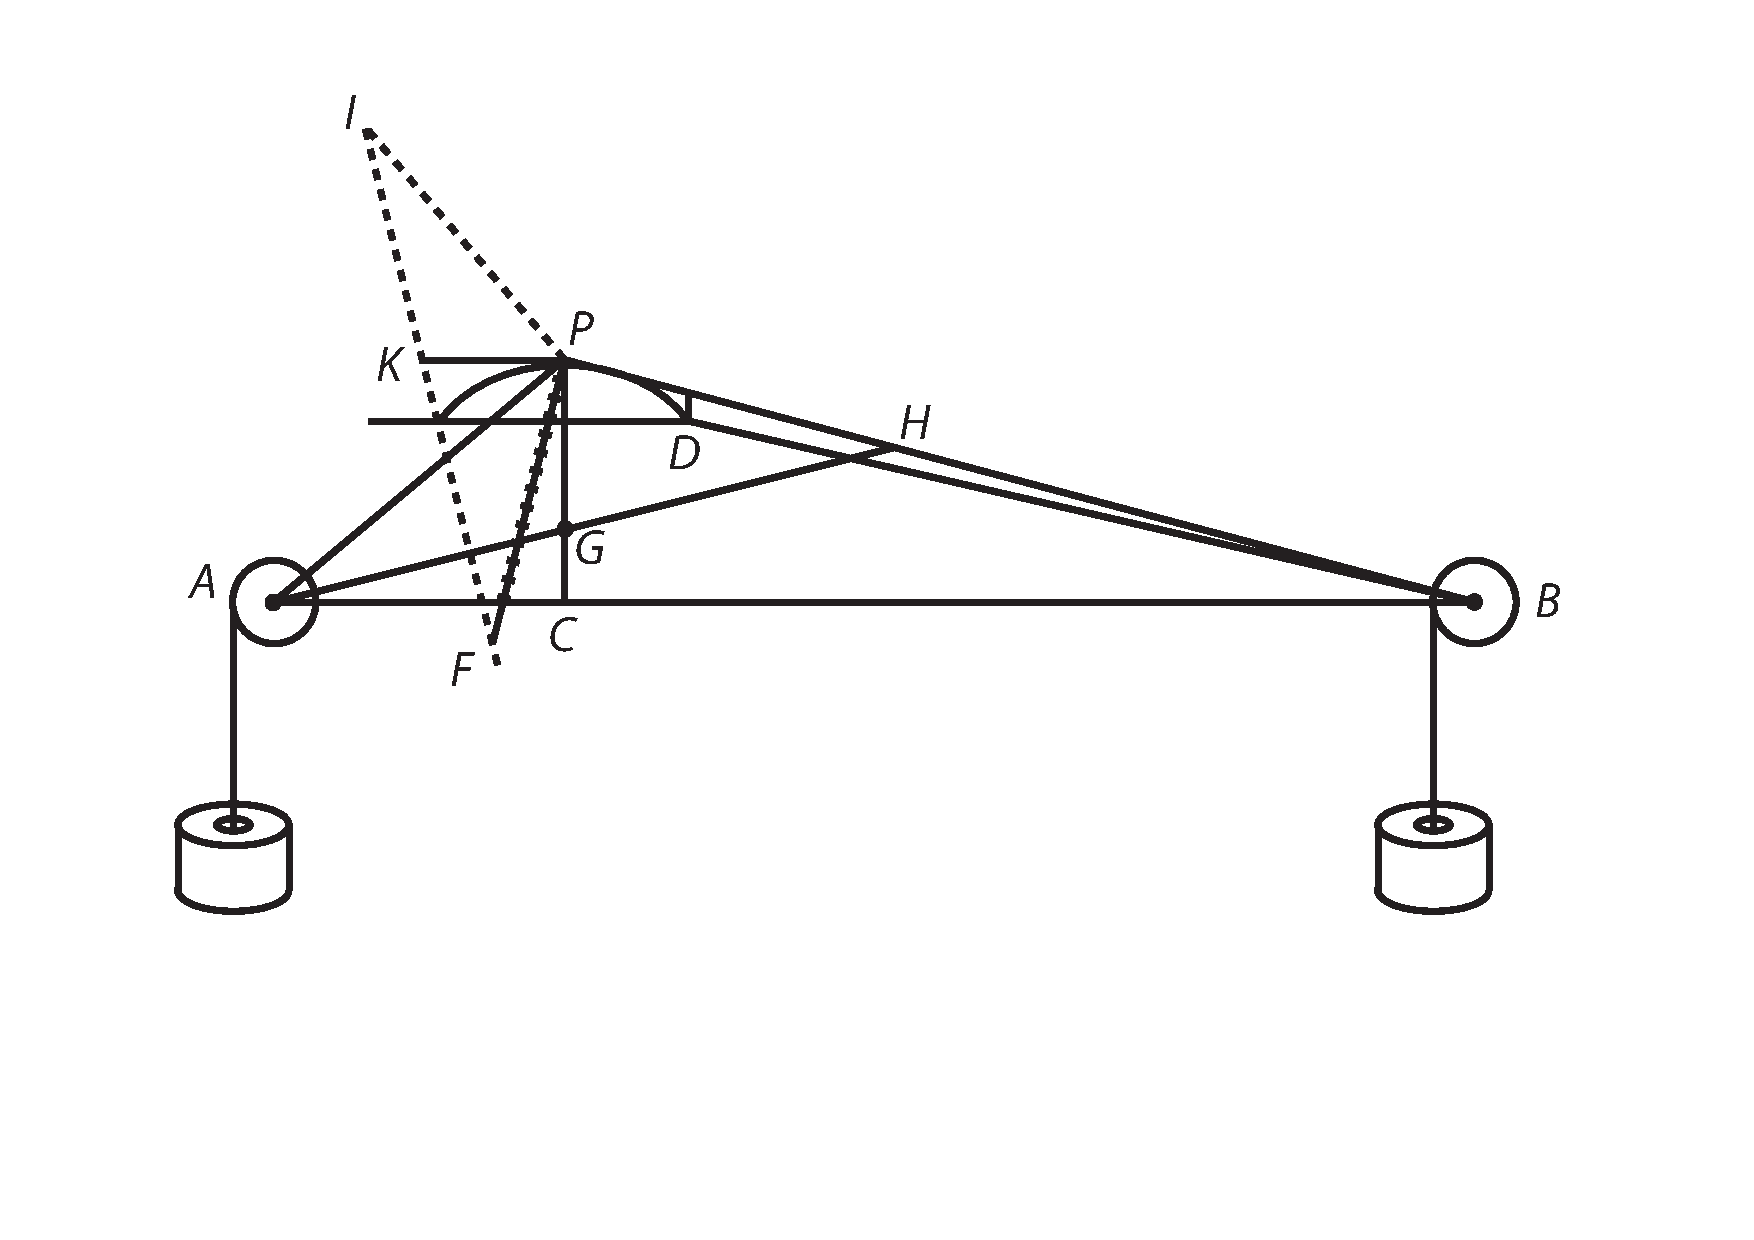
\includegraphics[width=0.83\textwidth]{images/LH03705_216v-d1.pdf}\\
\centering[\textit{Fig. 6}]
\pend
\newpage
\count\Afootins=1200
\count\Bfootins=1200
\count\Cfootins=1200
\pstart Radius $AP$ urget dentem curvam $EPD$ rotae $B$ in puncto aliquo, $P$. Dico quod perpendicularis contactus, (seu perpendicularis ad tangentem curvae) semper secat jungentem centra $AB$, in \textso{puncto $C$} ut motus rotae $B$ ad motum rotae $A$, \edtext{}{\lemma{}\Afootnote{\textit{Am Rand, gestrichen}: Hoc si verum esset curva necessario foret\textsuperscript{[a]} circularis.\\ {\footnotesize \textsuperscript{[a]} foret \textit{(1)}\ circulus \textit{(2)}\ circularis. \textit{L}}}} qui in nostro exemplo supponitur ut 1. ad 3. Fiat $PI$, aequalis et perpendicularis ipsi $AP$. 
\pend 
\pstart Ducatur $PB$ eique perpendicularis $PF$. Fiat $PH$ ad $PB$, ut revolutiones scilicet 1. ad 3. et fiat $PF$ aequalis $PH$. Ducatur $IF$ bisecta in $K$ ducatur item $AH$. \pend \pstart $P$ punctum describens curvam duos habet \edtext{motus, alterum circa}{\lemma{motus,}\Bfootnote{\textit{(1)}\ unum circa \textit{(2)}\ alterum circa \textit{L}}} centrum $A$, semidiametro $AP$, qui est in tangente $PI$, alterum qui est circa centrum $B$ semidiametro $BP$, qui est in tangente $PF$. Sed circa $A$ motus est triplo celerior quam circa $B$ ex constructione, sed quidem semidiametri essent aequales, sed ob earum inaequalitates tanto motus est celerior in $PF$ ac in $PI$ quanto $PB$ est major quam $PA$. Ut ex harum duarum rationum compositione celeritas in $PI$ sit ad illam in $PF$ ut $AP$ ad \rule[-4mm]{0mm}{10mm}$\displaystyle\frac{1}{3}$ $PB$ id est ad $PH$, seu ut $IP$ ad $\langle PF \rangle$. 
\pend 
\pstart Sed $IF$ est bissecta in $K$ ergo $KP$ est via puncti describentis, $P$; in dato momento, per Lemma I. quod idem est ac tangens. 
\pend 
\pstart Ulterius angulus $IPF$ est aeq. angulo $APH$ lineaeque $IP$, $AP$ aequales, item $PH$, \edtext{[$PF$]}{\lemma{$PE$}\Bfootnote{\textit{L \"{a}ndert Hrsg.}}} aequales. Ideoque $PC$ perpendicularis ad tangentem $KP$ bissecat $AH$ in $G$. Ideoque per Lemma II, ut $PH$ ad $PB$, sic $AC$, ad $CB$. Sed $PH$ ad $PB$ sunt revolutiones, ergo et haec, $AC$ scilicet ad $CB$. Quod erat ostendendum. \edtext{(+\phantom)\hspace{-1.2mm}  Haec obscuriuscule}{\lemma{(+\phantom)\hspace{-1.2mm}  Haec}\Bfootnote{\textit{(1)}\ paulo obscurius \textit{(2)}\ obscuriuscule \textit{ L}}} totidem verbis proposuit autor. [+)] 
\pend 
\pstart Notabile omnes curvae \edtext{motae}{\lemma{motae}\Bfootnote{\textit{erg. L}}} perpendiculares, semper cadere in \textso{punctum $C$}. \edtext{Adeoque si circulus}{\lemma{Adeoque}\Bfootnote{\textit{(1)}\ si diameter alicujus circulus mobilis intelligatur circa $C$ circulus autem diametro, semper per centrum transeunte sursum ac deorsum moveri possit; et circulus semper \textit{(2)}\ si circulus \textit{L}}} in curvae\edtext{}{\lemma{}\Afootnote{\textit{Am Rand, gestrichen}: Ergo curva foret circularis quod non puto.}} hujus concavitate moveri intelligatur, propellique ab ipso radio $AP$, ejus diameter semper transibit per $C$. Si planum quoddam cum ipso radio vel dente $BD$ circumagi intelligatur, in eo stylus $C$ fixus, utique circulum \edtext{describet. Cujus revolutio}{\lemma{describet.}\Bfootnote{\textit{(1)}\ Et semper quia $BC$, ad $AP$, in reciproca motuum ratione, nempe, motus ipsius puncti $P$  \textit{(a)}\ triplus \textit{(b)}\ seu extremi $P$, radii $P$, \textit{(aa)}\ triplus \textit{(bb)}\ revolutio tripla; ut contra radius $BC$, triplus radii $A$ \textit{(2)}\ Cujus revolutio \textit{L}}} aequalis revolutioni puncti $P$ circa $B$, et sub tripla ejusdem revolutioni circa $A$. Ponatur $AP$ \edtext{constans, quantalibet si esset $AP \sqcap AC$}{\lemma{constans,}\Bfootnote{\textit{(1)}\ aequalis $AC$ \textit{(2)}\ quantalibet [...] $AP \sqcap AC$. \textit{L}}}. Foret motus quo describeretur circulus in plano cum $B$ mobili, aequalis motui puncti $P$ circa $A$ sui inaequalis. Certe tamen in data ad id ratione erit.
\pend
\pstart
Eadem alia ratione et credo commodius invenientur, si uno centro fixo $A$, radio $AP$, describat circulum fixum. Dubito non videtur esse fixus. Imo est sed concipiendum est punctum $A$ simul circa centrum $B$ \setline{6}circumferri.
\pend
%\newpage% PR: Rein provisorisch !!!
\vspace*{2.5em}
\pstart
\centering
\noindent
%\begin{wrapfigure}{l}{0.3\textwidth}
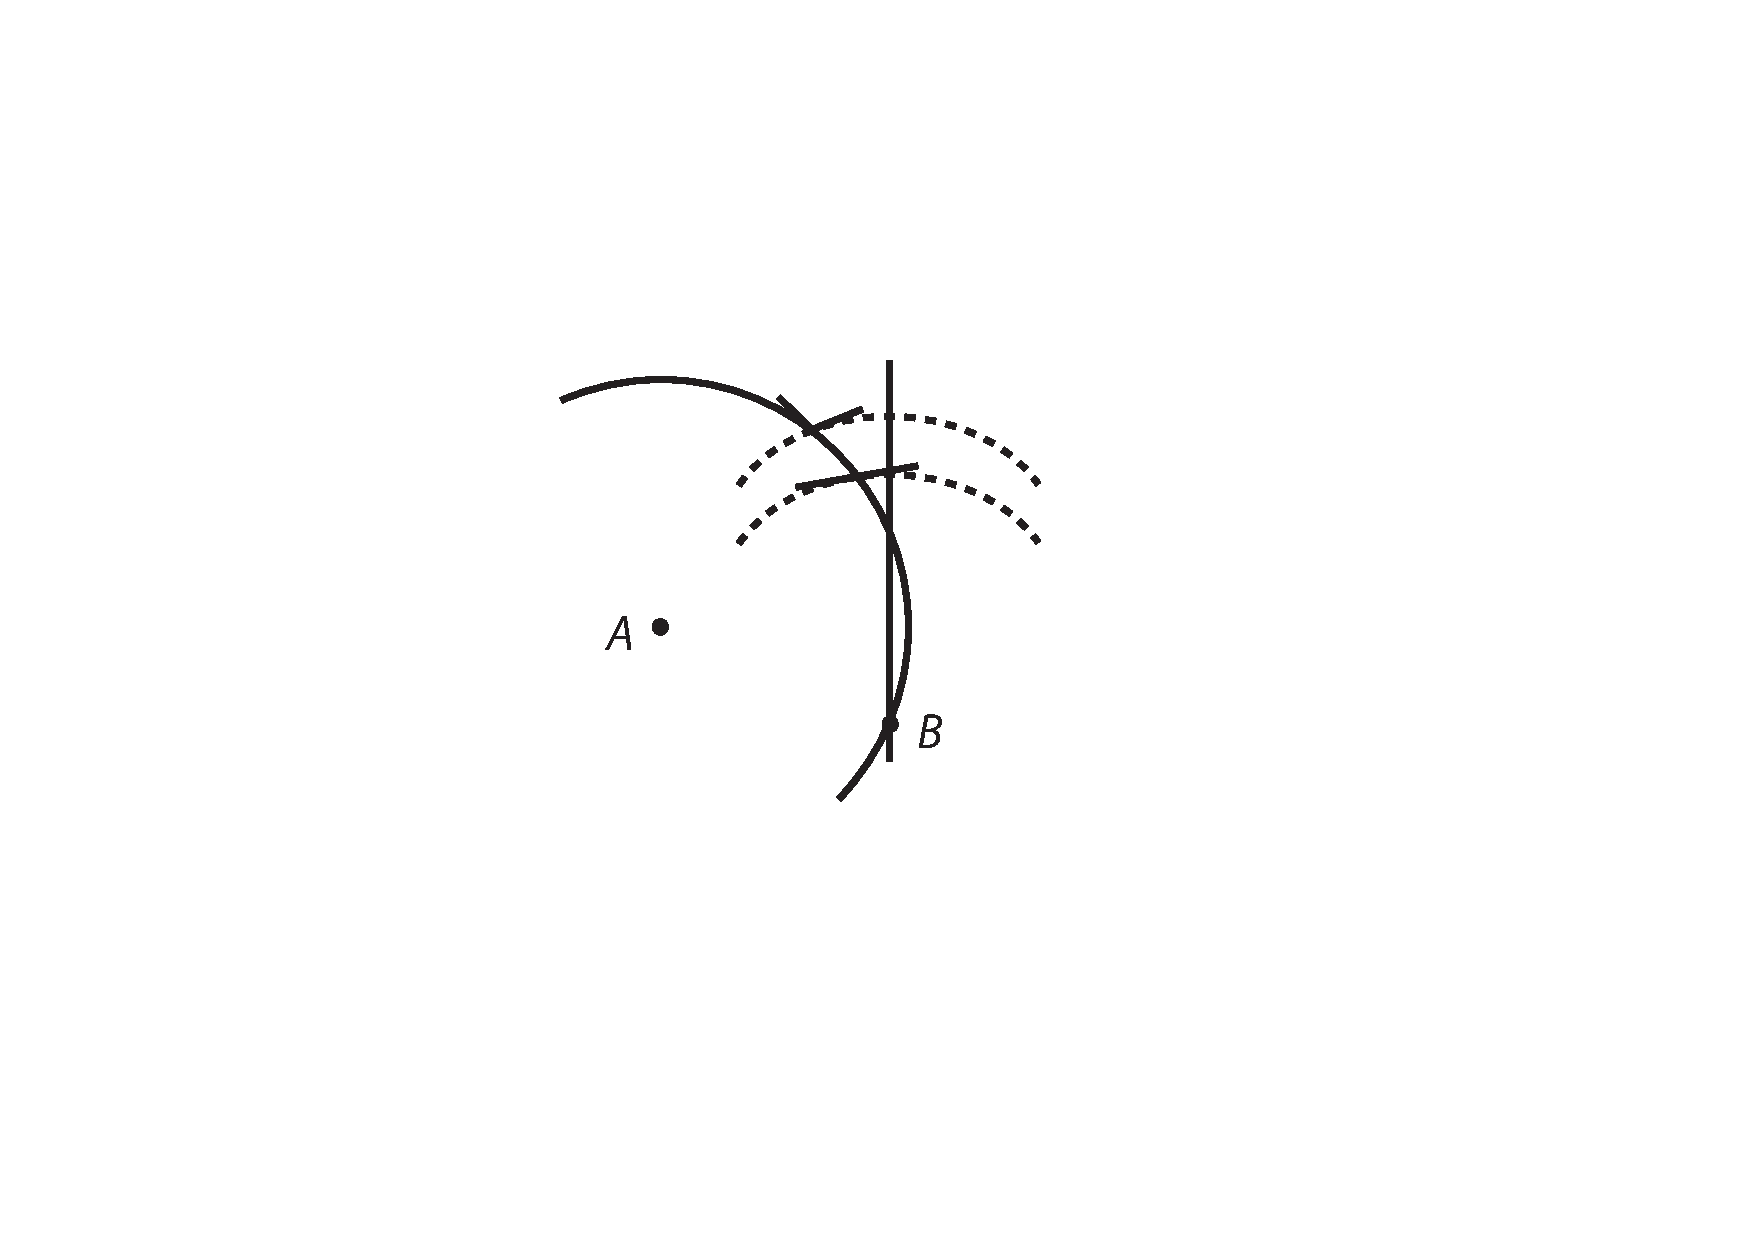
\includegraphics[width=0.31\textwidth]{images/LH03705_216v-d2.pdf}\\
\centering[\textit{Fig. 7}]
%\end{wrapfigure}
\pend
\count\Afootins=1500
\count\Bfootins=1500
\count\Cfootins=1500